%----------------------------------------------------------------------------
\chapter{Testing testing tools}\label{chapt:Testing tools}

\section{Garage Gate System Test Implementation}
\subsection{System implementation}
In order to discover different testing tools and environments, I have implemented the Garage Gate sample in c\# with Visual Studio and in java with Eclipse. In the \ref{subsect:Representation} section described the sample's state machine, which is quite straight-forward to implement, consequently I will focus in this section the known bugs in the code, which I want to detect by testing.
For testing goals by the implementation I have omitted some transitions from the state machine (see \figref{Garage Statemachine} figure), which were the loops (a transition which source and target state is the same), like in Closed state the closeSC and in Opening state the FreeMS.

\subsection{Test implementation}
\paragraph{GraphWalker test structure}
We can easily set up the GraphWalker test structure with Maven for our existing project. Then GraphWalker generate test cases from a graphml file, which is added to the project, thus I have created a graph representation matching the full functionalities of the SUT (see \figref{GraphWalker-GateModel} figure)

\begin{figure}[!ht]
	\centering
	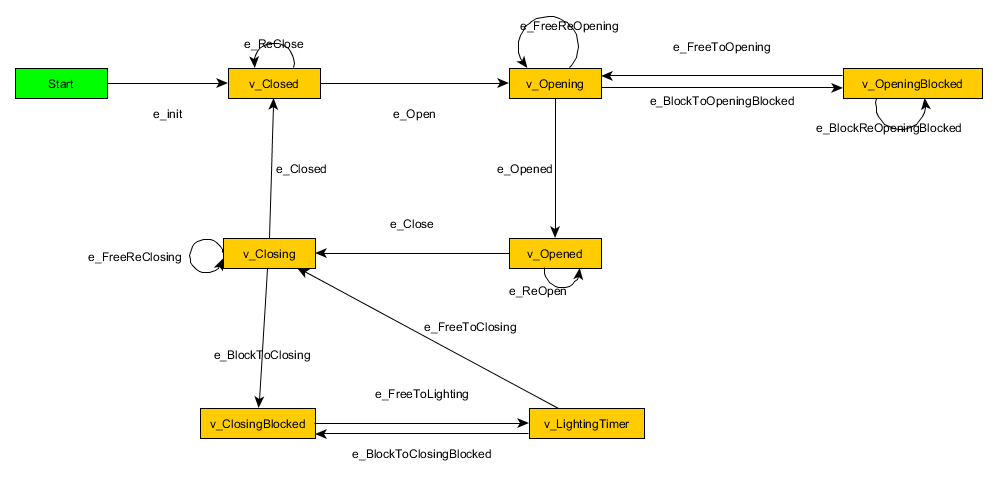
\includegraphics[width=150mm, keepaspectratio]{figures/GateModel.png}
	\caption{GraphWalker graph test model}
	\label{fig:GraphWalker-GateModel}
\end{figure}

With the \textit{graphwalker:generate-sources} command the tool have created an adaptation layer for our SUT. For testing purposes I configured \textit{GraphWalker} with the following annotation:
@GraphWalker(start = "e\_init", value = "quick\_random(edge\_coverage(80))").
With this command the test starts with the transition named "e\_init" and stops if the edge coverage value is above 80\%.
The tool supports several algorithm like quick\_random, random or a\_star.

In the adaptation code the recommended scenario is to have all commands to the SUT through the edge, and we assert our state in the vertexes.
\begin{minipage}{\linewidth}

Sample code snippet:
\begin{lstlisting}
@GraphWalker(start = "e_init", value = "quick_random(edge_coverage(80))")
public class GateModelTest extends ExecutionContext implements GateModel {
private GarageGateLogic gate;

@Override
public void e_BlockToOpeningBlocked() {
gate.setGateState(GarageGateState.OPENING);
gate.block();

}

@Override
public void v_Opening() {
Assert.expect(gate.getGateState()).equals(GarageGateState.OPENING);
}
\end{lstlisting}
\end{minipage}

\paragraph{SpecExplorer test structure}
SpecExplorer structure provides us 3 visual studio projects for testing purposes.
\begin{figure}[!ht]
	\centering
	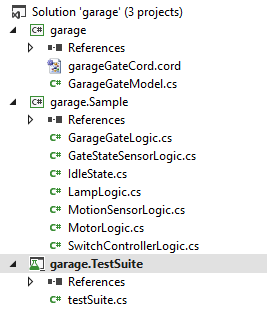
\includegraphics[width=50mm, keepaspectratio]{figures/specexplorerStructure.png}
	\caption{SpecExplorer Visual Studio testing structure}
	\label{fig:SpecExplorer Structure}
\end{figure}

\begin{itemize}
	\item \textbf{garage project:} Contains the configuration of SpecExplorer tool with cord files and belonging models.
	\item \textbf{garage.Sample:} This project can contain the whole implementation code (like in our case) or an test adapter which connects to the real SUT.
	\item \textbf{garage.TestSuite:} Unit test project. It is a result by test generation process.
\end{itemize}

To create a test suite which is satisfies our purposes, we need to create a finite cord file. 
First we list the available actions in a configuration:
\begin{lstlisting}
config Config 
{
	action abstract static void GarageGateLogic.openGate();
	action abstract static void GarageGateLogic.closeGate();
	action abstract static void GarageGateLogic.gateClosed();
	action abstract static void GarageGateLogic.gateOpened();
	action abstract static void GarageGateLogic.free();
	action abstract static void GarageGateLogic.block();
	
	switch StepBound = 128;
	switch PathDepthBound = 128;
	switch TestClassBase = "vs";
	switch GeneratedTestPath = "..\\garage.TestSuite";
	switch GeneratedTestNamespace = "garage.TestSuite";
	switch TestEnabled = false;
	switch ForExploration = false;
}
\end{lstlisting}

The next step is to create test-runnable machines for our needs, thus the state space get traversal by the following machine step by step:
\begin{lstlisting}
machine gateSteps() : Config where ForExploration = true
{
(openGate; free; block; free; gateOpened; closeGate; free; block; free; free; gateClosed;)*
}
machine testSuite() : Config where ForExploration = true, TestEnabled = true
{
construct test cases where Strategy = "ShortTests" for gateSteps() 
}
\end{lstlisting}


\begin{minipage}{\linewidth}
Our model file is calling the implementation from the garage project. Each action in the cord file can contract with a method in the model program. A sample code shown here:
\begin{lstlisting}
class GarageGateModel
{
private GarageGateState state;

[Rule(Action = "openGate()")]
public void openGate()
{
GarageGateLogic.openGate();
	state = GarageGateLogic.GateState;
}
\end{lstlisting}
\end{minipage}

We can now explorer and run our testSuite machine from the Exploration Manager. (see in \figref{SpecExpRun} figure)
\begin{figure}[!ht]
	\centering
	\includegraphics[width=100mm, keepaspectratio]{figures/specExplorerRun.png}
	\caption{Test environment in Visual Studio}
	\label{fig:SpecExpRun}
\end{figure}


\section{Testing results}
All the testing tools found the bugs in the implementation, which was consciously written by me. The \textit{SpecExplorer} gives direct navigation to the source code, where the exception was thrown, (see \figref{SpecExpRunFailed}). 
\begin{figure}[!ht]
	\centering
	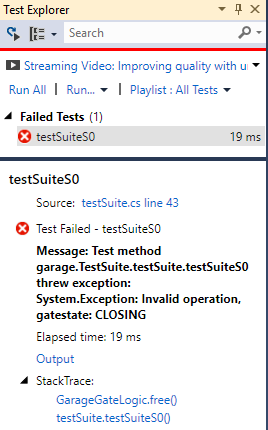
\includegraphics[width=50mm, keepaspectratio]{figures/specexplorerTestFailed.png}
	\caption{Test execution in Visual Studio}
	\label{fig:SpecExpRunFailed}
\end{figure}

The same error was found by \textit{GraphWalker} with random(edge\_coverage(80)) settings, and we can get detailed information about the failure:
\begin{lstlisting}
failures": [{"failure": "java.lang.RuntimeException\r\n\tat hu.bme.mit.GarageGate.GarageGateLogic.free(GarageGateLogic.java:78)\r\n\tat hu.bme.mit.GarageGate.GateModelTest.e_FreeReClosing(GateModelTest.java:88)\r\n\tat jdk.nashorn.internal.scripts.Script$Recompilation$22$369$\\^eval\\_.e_FreeReClosing(<eval>:1)\r\n\tat jdk.nashorn.internal.scripts.Script$21$\\^eval\\_.:program(<eval>:1)\r\n\tat jdk.nashorn.internal.runtime.ScriptFunctionData.invoke(ScriptFunctionData.java:637)\r\n\tat jdk.nashorn.internal.runtime.ScriptFunction.invoke(ScriptFunction.java:494)\r\n\tat jdk.nashorn.internal.runtime.ScriptRuntime.apply(ScriptRuntime.java:393)

"totalNumberOfModels": 1,
"totalCompletedNumberOfModels": 0,
"totalNumberOfVisitedEdges": 5,
"totalIncompleteNumberOfModels": 0,
"vertexCoverage": 57,
"totalNumberOfEdges": 16,
"totalNumberOfVisitedVertices": 4,
"edgeCoverage": 31,
"totalNumberOfVertices": 7,
"totalNumberOfUnvisitedEdges": 11
\end{lstlisting}

Interesting fact that with quick\_random(edge\_coverage(80)) setting the same bug was not found, with the same adaptation code and implementation, just with higher edge coverage percentage.
The Test result is:
\begin{lstlisting}
[INFO] Result :
[INFO] 
[INFO] {
"totalFailedNumberOfModels": 0,
"totalNotExecutedNumberOfModels": 0,
"totalNumberOfUnvisitedVertices": 0,
"verticesNotVisited": [],
"totalNumberOfModels": 1,
"totalCompletedNumberOfModels": 1,
"totalNumberOfVisitedEdges": 13,
"totalIncompleteNumberOfModels": 0,
"edgesNotVisited": [
{
"modelName": "GateModel",
"edgeId": "e2",
"edgeName": "e_FreeReClosing"
},
{
"modelName": "GateModel",
"edgeId": "e13",
"edgeName": "e_BlockReOpeningBlocked"
},
{
"modelName": "GateModel",
"edgeId": "e14",
"edgeName": "e_ReClose"
}
],
"vertexCoverage": 100,
"totalNumberOfEdges": 16,
"totalNumberOfVisitedVertices": 7,
"edgeCoverage": 81,
"totalNumberOfVertices": 7,
"totalNumberOfUnvisitedEdges": 3
}
[INFO] 
[INFO] ------------------------------------------------------------------------
[INFO] BUILD SUCCESS
[INFO] ------------------------------------------------------------------------
[INFO] Total time: 18.013 s
[INFO] Finished at: 2017-05-22T22:44:40+02:00
[INFO] Final Memory: 46M/446M
\end{lstlisting}


\paragraph{Reaching test goal}
In \textit{Spec Explorer} after detecting all the bugs in the implementation code, the test results in a passed state. (see \figref{SpecExpRunPassed}).
\begin{figure}[!ht]
	\centering
	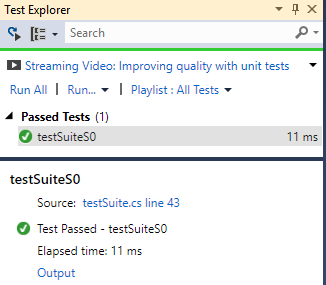
\includegraphics[width=50mm, keepaspectratio]{figures/specexplorerTestPassed.png}
	\caption{Test execution in Visual Studio}
	\label{fig:SpecExpRunPassed}
\end{figure}

In \textit{GraphWalker} with setup quick\_random(vertex\_coverage(100)) test settings the result was successful, although with random(vertex\_coverage(100)) the result was failure, because there were still missing loops in the implementation so there could be further development and investigating processes.

\begin{lstlisting}
quick\_random(vertex\_coverage(100))
[INFO] Result :
[INFO] 
[INFO] {
"totalFailedNumberOfModels": 0,
"totalNotExecutedNumberOfModels": 0,
"totalNumberOfUnvisitedVertices": 0,
"verticesNotVisited": [],
"totalNumberOfModels": 1,
"totalCompletedNumberOfModels": 1,
"totalNumberOfVisitedEdges": 8,
"totalIncompleteNumberOfModels": 0,
"edgesNotVisited": [
{
"modelName": "GateModel",
"edgeId": "e1",
"edgeName": "e_Closed"
},
{
"modelName": "GateModel",
"edgeId": "e2",
"edgeName": "e_FreeReClosing"
},
{
"modelName": "GateModel",
"edgeId": "e6",
"edgeName": "e_BlockToClosingBlocked"
},
{
"modelName": "GateModel",
"edgeId": "e7",
"edgeName": "e_FreeToClosing"
},
{
"modelName": "GateModel",
"edgeId": "e10",
"edgeName": "e_FreeReOpening"
},
{
"modelName": "GateModel",
"edgeId": "e13",
"edgeName": "e_BlockReOpeningBlocked"
},
{
"modelName": "GateModel",
"edgeId": "e14",
"edgeName": "e_ReClose"
},
{
"modelName": "GateModel",
"edgeId": "e15",
"edgeName": "e_ReOpen"
}
],
"vertexCoverage": 100,
"totalNumberOfEdges": 16,
"totalNumberOfVisitedVertices": 7,
"edgeCoverage": 50,
"totalNumberOfVertices": 7,
"totalNumberOfUnvisitedEdges": 8

****************************************************************************
random(vertex\_coverage(100))

[INFO] Result :
[INFO] 
[INFO] {
"totalFailedNumberOfModels": 0,
"totalNotExecutedNumberOfModels": 0,
"totalNumberOfUnvisitedVertices": 0,
"verticesNotVisited": [],
"totalNumberOfModels": 1,
"totalCompletedNumberOfModels": 1,
"totalNumberOfVisitedEdges": 14,
"totalIncompleteNumberOfModels": 0,
"edgesNotVisited": [
{
"modelName": "GateModel",
"edgeId": "e12",
"edgeName": "e_FreeToOpening"
},
{
"modelName": "GateModel",
"edgeId": "e13",
"edgeName": "e_BlockReOpeningBlocked"
}
],
"vertexCoverage": 100,
"totalNumberOfEdges": 16,
"totalNumberOfVisitedVertices": 7,
"edgeCoverage": 87,
"totalNumberOfVertices": 7,
"totalNumberOfUnvisitedEdges": 2
}
[INFO] 
[INFO] ------------------------------------------------------------------------
[INFO] BUILD SUCCESS

\end{lstlisting}

